\documentclass[t,aspectratio=169]{beamer}

\usepackage{soul}
\usepackage{multicol}
\usepackage[utf8]{inputenc}
\usepackage{amsmath}
\usepackage{physics}
\usepackage{siunitx}
\usepackage{graphicx}


% ----------------------------------------------------------------------------------------------------------------------------------------

\title{
\includegraphics[width=45pt]{oepecsetlogo.png}\\(KTXFI2EBNF) Physics II. Lecture}

\author{Dr.~Gábor FACSKÓ, PhD\\\tiny Assistant Professor / Senior Research Fellow\\\textit{facsko.gabor@uni-obuda.hu}}

\institute{\Tiny Óbuda University, Faculty of Electrical Engineering, 1084 Budapest, Tavaszmező u. 17.\\Wigner Research Centre for Physics, Department of Space Physics and Space Technology, 1121 Budapest, Konkoly-Thege Miklós út 29–33.\\ \url{https://wigner.hu/~facsko.gabor}}

\date{November~3,~2025}

\logo{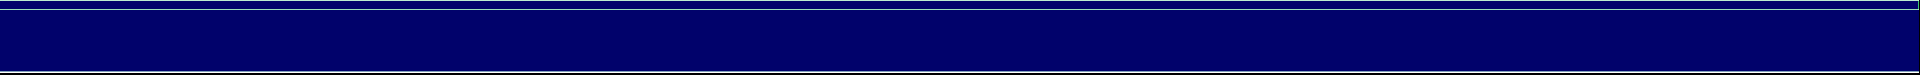
\includegraphics[height=0.9 true cm]{kekcsik.png}}

% ----------------------------------------------------------------------------------------------------------------------------------------

\begin{document}

\frame{\titlepage}

% ----------------------------------------------------------------------------------------------------------------------------------------

\begin{frame}%[fragile,squeeze,allowframebreaks]
\frametitle{Exams, Tests, etc.}
\begin{itemize}
\setlength{\parskip}{0pt}
\setlength{\itemsep}{0pt}
\item I had to announce the exams on short notice; therefore, you can take them on December 16, 2025, January 5, 19, and February 2, 2026, from 14:00 to 16:00.
\item The first exam is on a Tuesday, while the rest are on Mondays. You can also retake midterm tests and obtain your signature on December 16, 2025.
\medskip
\item You must take or retake the midterm exams before December 7, 2025. Therefore, I propose December 1, 2025, for the midterm exam and December 8, 2025, for the midterm retake.
\item I will give you your 2nd and 3rd homework assignments before December 1, 2025.
\item I currently have no idea when I will give you your 4th and 5th homework assignments\dots
\medskip
\item We will have lectures and practice sessions on November 3, 10, and 24, 2025.
\end{itemize}
\end{frame}


% ----------------------------------------------------------------------------------------------------------------------------------------

\begin{frame}[fragile,squeeze,allowframebreaks]
\frametitle{Where are we?}
\begin{itemize}
\setlength{\parskip}{0pt}
\setlength{\itemsep}{0pt}
\item \st{Motion of charged particles in electromagnetic fields.}
  \item \st{Elements of quantum mechanics. Heisenberg's uncertainty principle. The stationary Schrödinger equation and its applications.}
\item \st{Limits of the classical conceptual framework. Thermal radiation. Photoelectric effect. Compton effect. The dual nature of electromagnetic radiation. The dual nature of particles.}
\item \st{Moving reference frames. Inertial forces in accelerating reference frames. Elements of special relativity. Dirac-equation, antimatter.}
\item \st{The classical theory of atomic structure (Rutherford, Franck-Hertz experiment, Bohr model, quantum numbers, Pauli exclusion principle).}
\item \st{Physics of condensed matter. Metallic bonding. Electrical conduction in metals based on the free electron model and the wave model. Hall effect. Band theory of solids.}
\pagebreak
\item \textbf{Semiconductors. Elements of Fermi-Dirac statistics.} Thermoelectric phenomena. Magnetic properties.
\item Ferroelectricity. Piezoelectricity and electrostriction. Liquid crystals. Superconductivity.
\item Luminescence. Lasers. Basic knowledge of nuclear physics. Basic knowledge of particle physics.
\end{itemize}
\end{frame}

% ----------------------------------------------------------------------------------------------------------------------------------------

% Slide: Felvezetok_savelmelete_page01
\begin{frame}[fragile,squeeze,allowframebreaks]
\frametitle{Physical background of photovoltaic devices}
Silicon electron configuration: \texttt{$1s^2 2s^2 2p^6 3s^2 3p^2$}.
\begin{center}
\includegraphics[width=0.725\textwidth]{images-20251027/PeriodicTableECBlocks.png}
\end{center}

\pagebreak
\begin{center}
Photovoltaic devices — physical operating principles.\\
\includegraphics[width=0.45\textwidth]{images-20251103/aslide02_image04.png}
\end{center}

\pagebreak
\begin{center}
\includegraphics[width=0.45\textwidth]{images-20251103/aslide03_image01_modified.png}
\includegraphics[width=0.45\textwidth]{images-20251103/aslide03_image03.jpeg}
\end{center}
\end{frame}

% ----------------------------------------------------------------------------------------------------------------------------------------

% Slide: Felvezetok_savelmelete_page03
\begin{frame}[fragile,squeeze,allowframebreaks]
\frametitle{Charge carriers in semiconductors}
\begin{itemize}\setlength{\itemsep}{0pt}\setlength{\parskip}{0pt}
\item Electrons — mobile negative charge carriers in the conduction band.\medskip
\begin{center}
\includegraphics[width=0.7\textwidth]{images-20251103/aslide04_image04.png}
\end{center}

\pagebreak
\item Intrinsic (pure) semiconductor: silicon
\begin{itemize}\setlength{\itemsep}{0pt}\setlength{\parskip}{0pt}
\item Hole (positive charge carrier).
\item Valence electron and covalent bond formed by electron pairs.
\item Free electron (when a bond is broken by excitation).
\item Silicon atom lattice.
\medskip
\item Initial state (Silicon, Si): four valence electrons in covalent bonds; tetrahedral crystal structure.
\item Thermal excitation: covalent bonds may break, producing free electrons and enabling electrical current.
\item Holes: the vacant site left in the covalent bond when an electron is excited — a positive charge carrier.
\end{itemize}

\pagebreak
\item Band-to-band excitation and forbidden gap
\begin{columns}
\begin{column}{0.5\textwidth}
\begin{center}
\includegraphics[width=0.9\textwidth]{images-20251103/aslide05_image01.png}
\end{center}
\end{column}
\begin{column}{0.4\textwidth}
\begin{itemize}\setlength{\itemsep}{0pt}\setlength{\parskip}{0pt}
\item Electrons can be excited from the valence band (A) into the conduction band (V) by sufficient energy input.
\item Electrons can never occupy states within the forbidden gap (T).
 \end{itemize}
\end{column}
\end{columns}

\pagebreak
\item Extrinsic (doped) semiconductors
\begin{itemize}\setlength{\itemsep}{0pt}\setlength{\parskip}{0pt}
\item p-type doping: acceptor levels near the valence band introduce holes (positive carriers).
\item n-type doping: donor levels near the conduction band introduce extra electrons (negative carriers).
\end{itemize}
\begin{center}
\includegraphics[width=0.525\textwidth]{images-20251103/aslide06_image04.png}
\end{center}

\pagebreak
\item n-type doping and donor levels
\begin{columns}
  \begin{column}{0.6\textwidth}
\begin{center}
\includegraphics[width=0.9\textwidth]{images-20251103/aslide07_image04.png}
\end{center}
\end{column}
\begin{column}{0.4\textwidth}    
\begin{itemize}\setlength{\itemsep}{0pt}\setlength{\parskip}{0pt}
\item In n-type doping, donor levels form close to the conduction band edge. Electrons introduced by the dopant occupy these donor levels.
\item These donor electrons are more easily thermally excited into the conduction band where they act as free charge carriers and contribute to electrical conduction.
\end{itemize}
\end{column}
\end{columns}

\pagebreak
\item p-type doping and acceptor levels
\begin{columns}
  \begin{column}{0.55\textwidth}
\begin{center}
\includegraphics[width=0.9\textwidth]{images-20251103/aslide08_image04.png}
\end{center}
\end{column}
\begin{column}{0.45\textwidth}    
\begin{itemize}\setlength{\itemsep}{0pt}\setlength{\parskip}{0pt}
\item In p-type doping, acceptor levels form near the top of the valence band. The holes introduced by the dopant occupy those acceptor levels.
\item These holes can recombine with electrons in the valence band or facilitate excitation of valence electrons into the acceptor level more easily than into the conduction band, due to the smaller energetic separation (smaller local gap).
\end{itemize}
\end{column}
\end{columns}

\pagebreak
\item By combining p-type and n-type semiconductors, a diode can be formed. When the cathode is connected to the n-type semiconductor and the anode to the p-type semiconductor, charge carriers accumulate near the junction, allowing current to flow (forward bias). In the reverse direction (reverse bias), the current is effectively blocked.
\smallskip
\begin{center}
  \includegraphics[width=0.3\textwidth]{images-20251103/diode01.png}
  \includegraphics[width=0.3\textwidth]{images-20251103/diode02.png}
  \includegraphics[width=0.3\textwidth]{images-20251103/diode03.png}
\end{center}
\smallskip

\item Very small electronic circuits (down to the $\sim\,$nm scale) can be manufactured using these semiconductor materials.

\pagebreak
\item By connecting two diodes in opposite orientation, a transistor can be constructed.
\begin{columns}
  \begin{column}{0.4\textwidth}
    \begin{center}
      \includegraphics[width=0.3\textwidth]{images-20251103/transistor-construction.png}
    \end{center}
  \end{column}
  \begin{column}{0.5\textwidth}    
    \begin{itemize}\setlength{\itemsep}{0pt}\setlength{\parskip}{0pt}
      \item Both \textit{npn} and \textit{pnp} transistors can be realized.
      \item By applying a potential difference between the emitter and the base, the current through the device can be controlled; effectively, the transistor acts as an electronic switch.
      \item These transistors can also be fabricated at extremely small dimensions (down to the $\sim\,$nm scale).
    \end{itemize}
  \end{column}
\end{columns}

\end{itemize}
\end{frame}

% Now slides from Fermi-Dirac PDF (multiple pages)

\begin{frame}[fragile,squeeze,allowframebreaks]
\frametitle{Elements of Fermi--Dirac statistics}
\begin{itemize}\setlength{\itemsep}{0pt}\setlength{\parskip}{0pt}
\item Basics of Fermi--Dirac statistics
\begin{itemize}\setlength{\itemsep}{0pt}\setlength{\parskip}{0pt}
\item For systems with a large number of particles, statistical descriptions are required to characterize their physical properties (similar to classical statistics for gases).
\item Electrons behave analogously to gas particles in such statistical descriptions.
\item Enrico Fermi developed the model for fermions in 1920 (Rome).
\item Applies to fermions (half-integer spin particles), including electrons.
\end{itemize}

\item Assumptions of Fermi--Dirac statistics
\begin{itemize}\setlength{\itemsep}{0pt}\setlength{\parskip}{0pt}
\item Particles are indistinguishable.
\item Energy levels are quantized (Bohr postulates apply).
\item Pauli exclusion principle: no more than one fermion (per spin state) can occupy the same quantum state.
\item Heisenberg uncertainty relations limit phase-space cell size: $\Delta p\cdot \Delta x$ defines a phase-space cell volume.
\end{itemize}

\pagebreak
\item Fermi distribution function
\begin{columns}
  \begin{column}{0.225\textwidth}
\begin{center}
\includegraphics[width=0.9\textwidth]{images-20251103/bslide06_image02.png}
\end{center}
\end{column}
\begin{column}{0.45\textwidth}    
\begin{equation*}
P(W)=\frac{1}{\exp\!\left(\frac{W-W_F}{kT}\right)+1}
\end{equation*}
\begin{itemize}\setlength{\itemsep}{0pt}\setlength{\parskip}{0pt}
\item $W_F$: Fermi energy (to be defined).
\item $k$: Boltzmann constant. $W$: energy level. $T$: absolute temperature (K).
\end{itemize}
\end{column}
\end{columns}

\pagebreak
\item Interpretation of the Fermi function
\begin{columns}
  \begin{column}{0.6\textwidth}
\begin{center}
\includegraphics[width=0.9\textwidth]{images-20251103/bslide07_image01.jpeg}
\end{center}
\end{column}
\begin{column}{0.4\textwidth}    
\begin{itemize}\setlength{\itemsep}{0pt}\setlength{\parskip}{0pt}
\item The Fermi function gives the probability that an energy level $W$ is occupied by an electron.
\item At $T=0\,$K, $f(W)=1$ for $W<W_F$, and $f(W)=0$ for $W>W_F$.
\item At $T>0\,$K, $f(W_F)=\tfrac{1}{2}$.
\end{itemize}
\end{column}
\end{columns}

\pagebreak
\item Density of available states $S'(W)$
\begin{columns}
  \begin{column}{0.6\textwidth}
\begin{center}
\includegraphics[width=0.9\textwidth]{images-20251103/bslide08_image02.png}
\end{center}
\end{column}
\begin{column}{0.4\textwidth}  
\begin{itemize}\setlength{\itemsep}{0pt}\setlength{\parskip}{0pt}
\item $S'(W)$ denotes the density of available single-particle quantum states per unit volume as a function of energy $W$.
\item Physically: the number of distinct quantum states (e.g., seats in a theater analogy) available at a given energy.
\end{itemize}
\end{column}
\end{columns}

\pagebreak
\item Energy distribution density function
\begin{equation*}
\frac{dn}{dW}=4\pi\left(2m\right)^{3/2}\!/\!h^3 \;\cdot\; \frac{1}{\exp\!\left(\frac{W-W_F}{kT}\right)+1}\; \cdot\; W^{1/2}
\end{equation*}
This function describes how electrons populate energy levels per unit energy interval and per unit volume.
\begin{center}
\includegraphics[width=0.4\textwidth]{images-20251103/bslide10_image01.jpeg}
\end{center}

\pagebreak
\item Separation and integration of the distribution
\begin{itemize}\setlength{\itemsep}{0pt}\setlength{\parskip}{0pt}
\item The differential form: $dn = \left[4\pi(2m)^{3/2}/h^3\right]\frac{1}{e^{(W-W_F)/kT}+1} W^{1/2}\,dW$.
\item Integrating from 0 to $W_F^0$ at $T=0$ K yields the electron concentration $n$ and the zero-temperature Fermi energy $W_F^0$.
\end{itemize}
\item{Zero-temperature Fermi energy}
\begin{equation*}
S\left(W\right)=W_F^0=\frac{3n}{8\pi}\left(\frac{h^2}{2m}\right)\!^{\!2/3}
\end{equation*}
\item The zero-temperature Fermi energy depends only on the conduction electron concentration $n$ and fundamental constants.

\end{itemize}
\end{frame}

% ----------------------------------------------------------------------------------------------------------------------------------------

\begin{frame}[fragile,squeeze,allowframebreaks]
  \frametitle{Work function and potential energy reference}
  \begin{itemize}
  \item Work function
\begin{columns}
  \begin{column}{0.6\textwidth}
\begin{center}
\includegraphics[width=0.9\textwidth]{images-20251103/bslide13_image01.png}
\end{center}
\end{column}
\begin{column}{0.4\textwidth}  
\begin{itemize}\setlength{\itemsep}{0pt}\setlength{\parskip}{0pt}
\item The potential energy of an electron bound to the atomic nucleus is negative; at infinite separation it approaches zero.
\item Inside a metal the potential energy of free electrons, $W_0$, is negative and rises toward the surface, becoming zero outside the metal.
\end{itemize}
\end{column}
\end{columns}

\pagebreak
\item Kinetic energy in the conduction band and Fermi level
  \begin{columns}
  \begin{column}{0.6\textwidth}
 \begin{center}
\includegraphics[width=0.65\textwidth]{images-20251103/bslide14_image01.png}
\end{center}
\end{column}
\begin{column}{0.4\textwidth}  
\begin{itemize}\setlength{\itemsep}{0pt}\setlength{\parskip}{0pt}
\item Electrons in the conduction band possess kinetic energy in addition to potential energy; their kinetic energy distribution depends on the electron population.
\item Definition (Fermi level): the energy level corresponding to electrons with the highest occupied kinetic energy at $T=0$ K.
\end{itemize}
\end{column}
\end{columns}

\pagebreak
\item Fermi level occupancy and work function
 \begin{columns}
  \begin{column}{0.6\textwidth}
 \begin{center}
\includegraphics[width=0.9\textwidth]{images-20251103/bslide15_image01.png}
\end{center}
\end{column}
\begin{column}{0.4\textwidth}  
\begin{itemize}\setlength{\itemsep}{0pt}\setlength{\parskip}{0pt}
\item At $T=0$ K all states below the Fermi level are fully occupied; states above are empty.
\item Definition (work function): the energy $W_k$ required to remove an electron at the Fermi level from the metal. It equals the absolute value of the potential energy $W_0$ plus the Fermi energy difference:
\end{itemize}
\begin{equation*}
W_k = W_0 - W_F
\end{equation*}
\end{column}
\end{columns}

\end{itemize}
\end{frame}



% ----------------------------------------------------------------------------------------------------------------------------------------

\begin{frame}
%\frametitle{Minden jó, ha a vége jó}

\vfill
\begin{center}
\textbf{\huge The End}

\bigskip
Thank you for your attention!
\end{center}
\vfill
\end{frame}

\end{document}
